\section{Parallel Computing, the GPU Architecture and OpenCL}

As CPU clock speeds started to reach an upper bound of feasibility in
about 2004~\cite{clockspeed}, processor manufacturers started to look
for new ways to increase the speed of computation in
computers. Parallelization quickly proved to offer speedups in form of
parallel computations. The idea is simple: use two or more cores in
parallel to work on different aspects of a problem and merge the
results in an effective manner.

As an example, suppose that we want to increment all elements in an
array of $n$ integers by one. Using a traditional CPU would require
$n$ sequential operations on the array, but if two traditional CPUs
could somehow share the memory between them, then one of the CPUs
could process one half of the array, while the other CPU processes the
other half at the same time. We still require $n$ operations on the
array, but it only takes half the time.

\subsection{Parallel architectures}

Of course, many different parallel architectures exist, with
individual scales and applications.

\emph{Grid computing systems}, where computation takes places across
multiple independent administrative domains, offer the largest scale
of parallel computing. Typically, grids, as they are also called, are
comprised of many different devices owned by seperate entities, who
pool their resources together. A famous example of grid computing is
the SETI@home project~\cite{seti}, where hundreds of thousands of
people around the globe connect over the internet to volunteer their
computer resources towards the search for extraterrestrial
life~\cite{seti-number}. The project has since spawned the BOINC
grid-computing framework, which is used to research things like
protein folding \cite{boinc-other} using the same techniques. These
systems offer massive computational power, at the cost of low speed of
transfer, as well as the need to have a central server delegate
sub-tasks to the individual participants in the grid. As a result of
the low speed of transfer, the sub-tasks must be relatively
independent, and require a high-time-of-computation to data-size
ratio, for grids to be efficient.

\emph{MMP (Massively Parallel Processor) systems}, commonly associated
with supercomputers, frequently take up entire storage
facilities~\cite{supercomputer-size}, and are composed of thousands of
processors connected via highly specialized interfaces that have been
constructed specifically for the purpose of the supercomputer. They
typically offer very high computational power, much better
communication between processors than grids, but at an enormous
cost~\cite{supercomputer-cost}. These machines are typically owned by
government institutions and agencies, and are used for research, in
the military, as well as in meteorological
computations~\cite{supercomputer-use}.

\emph{Cluster server systems}, are composed of multiple general
purpose computers that share computational resources and data across a
specialized network. Typically used for application servers in
businesses~\cite{clusters-in-business}, they are not quite as
expensive as supercomputers, but provide a significant boost in power
compared to traditional servers, as well as the ability to provide
redundancy and fail-over services.

\emph{Symmetric multiprocessing (SMP) systems}, are traditional
computers containing multiple identical processors connected as a
single unit~\cite{smp}. Examples of these include Intel Core 2 Duo
processors, which is actually comprised of two Intel Core 2 processors
acting in unison~\cite{intelcore2duo}. Some of the first experiments
with parallel architectures for consumer PCs are examples of SMP
systems. In fact, at a certain point, some motherboards had two CPU
sockets, allowing the user to install an additional identical CPU for
a speed boost~\cite{two-cpus}.

\emph{Multi-core processors}, consist of a single chip with more than
one computing core. Many modern CPUs contain more than a single core,
the Intel Core 2 processor, for example, contains 2~\cite{intelcore2},
but multi-core processors are commonly associated with video
cards. Video cards include one or more \emph{GPUs (Graphical
  Processing Units)}, which is a multi-core processor specifically
designed for certain parallel kinds of operations pertaining to
graphics processing. Originally designed and sold to consumers to
enhance 3-D graphics in video games, because of their parallel
architecture, GPUs have since found many other applications.

\subsection{Graphical Processing Units}

Modern GPUs include hundreds or thousands of cores that all can be
used in parallel to effectively perform such things as matrix
operations and operations on large arrays; when it comes to these
kinds of operations GPUs offer huge speed gains compared to
traditional CPUs, at an affordable price.

GPU architectures, such as NVIDIAs Kepler GK110, typically consist of
a number of cores, grouped in some number of groups. On top of an
amount of shared memory between all groups, each group has its own
memory, that all cores in the group can uniformly access.

\begin{figure}
  \centering
  \caption{Diagram of NVIDIAs Kepler GK110 architecture}
  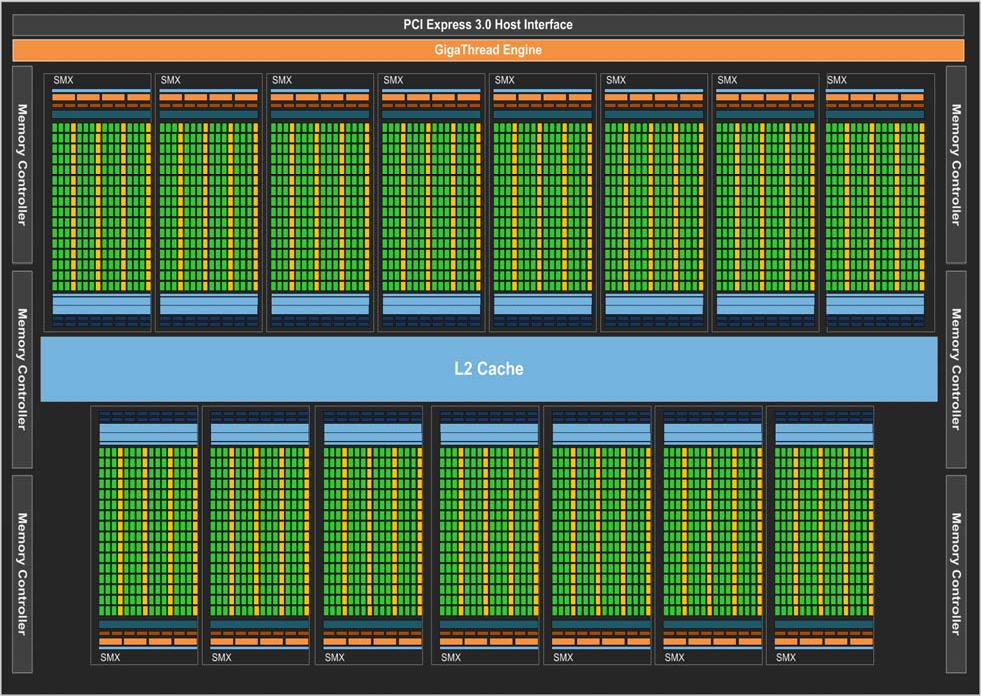
\includegraphics[width=1\textwidth]{figures/kepler110.png}
  \label{kepler}
\end{figure}

As an example, the Kepler GK110 is equipped with 15 groups of cores,
called \emph{Streaming Multiprocessors (SMX)}, each with 192
single-precision cores, and 64 double-precision cores and several
other cores for more specific operations~\cite{kepler}. Each streaming
multiprocessor has 64 KB of memory that is shared between its cores,
in addition to 1536 KB memory that is shared between all of the
streaming multiprocessors.

In order to efficiently take advantage of all this parallel processing
power, special care must be taken when programming for the GPU. We
have to efficiently divide the work into parts, distribute them across
groups and cores, make sure that cores do not overwrite the work of
each other, synchronize results and so on. Luckily, frameworks, such
as \emph{OpenCL}, can help us with these tasks~\footnote{CUDA is
  another popular framework, specifically for programming NVIDIA
  GPUs. While Smlcl will focus on GPU programming, we also want to
  allow other GPUs than NVIDIAs, which is why we've chosen to work
  with OpenCL}.

\subsection{OpenCL}

Originally created by the non-profit technology consortium Khronos
Group~\cite{khronos}, and since embraced by numerous hardware and
software companies, including AMD and NVIDIA, the two biggest
manufacturers of GPUs, OpenCL is ``a framework suited for parallel
programming of heterogeneous systems''~\cite{opencl-quote}. With it,
you can write programs that runs uniformly on both CPUs and GPUs, as
well as Digital Signal Processors and other kinds processors
supporting the framework, allowing you to take advantage of many
different architectures using the same code.

In OpenCL, programs are made up of \emph{kernels}, which are written
in a C-like language and some host code. Each kernel takes a set of
arguments, performs some kind of computation, and modifies one or more
of the arguments to include the result (in OpenCL, kernels cannot
return values, therefore results are returned to the caller via
in-memory data-structures). \emph{Work groups} are made up of a number
of kernels, and arguments to kernels can be either global (all kernels
access the same memory), local (only kernels in the same work group
can access the same memory) or private (no other kernel can access
this memory). Each kernel also has a unique global ID, a work group
ID, and a unique ID within it's work group.

The host code, typically written in C or C++~\cite{hostlang}, uses the
OpenCL API to set up the OpenCL environment for a specific device,
compile and build the kernel code, transfer data to buffers on the
device, execute the kernels and read the results back from the
buffers. Appendix \ref{vectoradd}, shows the code required to
calculate the addition of two vectors. As it can be seen, even
executing a rather simple computation like a vector addition, takes
many steps, and there is a high risk of introducing errors when
writing the code, simply because of the complexity of the process.
